\clearpage
\makeatletter
\efloat@restorefloats
\makeatother


\begin{appendix}
\hypertarget{sa-confirming-the-five-factor-solution-obtained-using-minimum-residual-extraction-method}{%
\section{SA: Confirming the five factor solution obtained using minimum
residual extraction
method}\label{sa-confirming-the-five-factor-solution-obtained-using-minimum-residual-extraction-method}}

\begin{center}
\begin{ThreePartTable}

\begin{TableNotes}[para]
\normalsize{\textit{Note.} Only loading higher than .30 is reported}
\end{TableNotes}

\begin{longtable}{llllllll}\noalign{\getlongtablewidth\global\LTcapwidth=\longtablewidth}
\caption{\label{tab:MinResTab}Factor loadings and communality of the retained items(Minmum Residual)}\\
\toprule
item & \multicolumn{1}{c}{MR1} & \multicolumn{1}{c}{MR2} & \multicolumn{1}{c}{MR3} & \multicolumn{1}{c}{MR4} & \multicolumn{1}{c}{MR5} & \multicolumn{1}{c}{Communality} & \multicolumn{1}{c}{Uniqueness}\\
\midrule
\endfirsthead
\caption*{\normalfont{Table \ref{tab:MinResTab} continued}}\\
\toprule
item & \multicolumn{1}{c}{MR1} & \multicolumn{1}{c}{MR2} & \multicolumn{1}{c}{MR3} & \multicolumn{1}{c}{MR4} & \multicolumn{1}{c}{MR5} & \multicolumn{1}{c}{Communality} & \multicolumn{1}{c}{Uniqueness}\\
\midrule
\endhead
item16 & 1 &  &  &  &  & 0.996 & 0.004\\
item36 & 0.94 &  &  &  &  & 0.897 & 0.103\\
item17 & 0.8 &  &  &  &  & 0.658 & 0.342\\
item11 &  & 0.79 &  &  &  & 0.642 & 0.358\\
item10 &  & 0.76 &  &  &  & 0.592 & 0.408\\
item12 &  & 0.65 &  &  &  & 0.465 & 0.535\\
item7 &  & 0.5 &  &  &  & 0.267 & 0.733\\
item8 &  & -0.49 &  &  &  & 0.252 & 0.748\\
item9 &  & 0.32 &  &  &  & 0.113 & 0.887\\
item27 &  &  & 0.8 &  &  & 0.659 & 0.341\\
item3 &  &  & 0.8 &  &  & 0.683 & 0.317\\
item40 &  &  & 0.65 &  &  & 0.464 & 0.536\\
item30 &  &  & 0.45 &  &  & 0.353 & 0.647\\
item41 &  &  & 0.36 &  &  & 0.329 & 0.671\\
item33 &  &  &  & 0.74 &  & 0.555 & 0.445\\
item32 &  &  &  & 0.73 &  & 0.623 & 0.377\\
item35 &  &  &  & 0.66 &  & 0.455 & 0.545\\
item37 &  &  &  & -0.39 &  & 0.175 & 0.825\\
item38 &  &  &  & 0.38 &  & 0.178 & 0.822\\
item46 &  &  &  &  & 0.6 & 0.422 & 0.578\\
item45 &  &  &  &  & 0.59 & 0.374 & 0.626\\
item25 &  &  &  &  & 0.41 & 0.193 & 0.807\\
item4 &  &  &  &  & 0.41 & 0.219 & 0.781\\
item1 &  &  &  &  & 0.4 & 0.17 & 0.83\\
item26 &  &  &  &  & 0.35 & 0.165 & 0.835\\
\% of Variance & 0.1 & 0.1 & 0.09 & 0.08 & 0.06 &  & \\
\bottomrule
\addlinespace
\insertTableNotes
\end{longtable}

\end{ThreePartTable}
\end{center}

\hypertarget{sa-factor-analysis-with-six-factors}{%
\section{SA: Factor analysis with six
factors}\label{sa-factor-analysis-with-six-factors}}

\begin{center}
\begin{ThreePartTable}

\begin{TableNotes}[para]
\normalsize{\textit{Note.} Only loading higher than .30 is reported}
\end{TableNotes}

\begin{longtable}{lllllllll}\noalign{\getlongtablewidth\global\LTcapwidth=\longtablewidth}
\caption{\label{tab:sixFacTab}Factor loadings and communality of the retained items(six factor)}\\
\toprule
item & \multicolumn{1}{c}{PA1} & \multicolumn{1}{c}{PA4} & \multicolumn{1}{c}{PA2} & \multicolumn{1}{c}{PA3} & \multicolumn{1}{c}{PA5} & \multicolumn{1}{c}{PA6} & \multicolumn{1}{c}{Communality} & \multicolumn{1}{c}{Uniqueness}\\
\midrule
\endfirsthead
\caption*{\normalfont{Table \ref{tab:sixFacTab} continued}}\\
\toprule
item & \multicolumn{1}{c}{PA1} & \multicolumn{1}{c}{PA4} & \multicolumn{1}{c}{PA2} & \multicolumn{1}{c}{PA3} & \multicolumn{1}{c}{PA5} & \multicolumn{1}{c}{PA6} & \multicolumn{1}{c}{Communality} & \multicolumn{1}{c}{Uniqueness}\\
\midrule
\endhead
item19 & 1.78 &  &  &  &  &  & 3.318 & -2.318\\
item5 &  &  &  &  &  &  & 0.11 & 0.89\\
item16 &  & 1 &  &  &  &  & 1.004 & -0.004\\
item36 &  & 0.91 &  &  &  &  & 0.86 & 0.14\\
item17 &  & 0.81 &  &  &  &  & 0.691 & 0.309\\
item11 &  &  & 0.83 &  &  &  & 0.71 & 0.29\\
item10 &  &  & 0.79 &  &  &  & 0.638 & 0.362\\
item12 &  &  & 0.63 &  &  &  & 0.465 & 0.535\\
item8 &  &  & -0.5 &  &  &  & 0.269 & 0.731\\
item7 &  &  & 0.47 &  &  &  & 0.268 & 0.732\\
item9 &  &  & 0.32 &  &  &  & 0.163 & 0.837\\
item33 &  &  &  & 0.83 &  &  & 0.698 & 0.302\\
item32 &  &  &  & 0.75 &  &  & 0.666 & 0.334\\
item35 &  &  &  & 0.64 &  &  & 0.446 & 0.554\\
item31 &  &  &  & 0.48 &  &  & 0.331 & 0.669\\
item38 &  &  &  & 0.39 &  &  & 0.191 & 0.809\\
item37 &  &  &  & -0.35 &  &  & 0.153 & 0.847\\
item3 &  &  &  &  & 0.85 &  & 0.748 & 0.252\\
item27 &  &  &  &  & 0.8 &  & 0.644 & 0.356\\
item40 &  &  &  &  & 0.68 &  & 0.507 & 0.493\\
item46 &  &  &  &  &  & 0.6 & 0.431 & 0.569\\
item45 &  &  &  &  &  & 0.56 & 0.341 & 0.659\\
item4 &  &  &  &  &  & 0.43 & 0.265 & 0.735\\
item25 &  &  &  &  &  & 0.4 & 0.178 & 0.822\\
item1 &  &  &  &  &  & 0.36 & 0.142 & 0.858\\
item26 &  &  &  &  &  & 0.36 & 0.173 & 0.827\\
item13 &  &  &  &  &  &  & 0.087 & 0.913\\
item29 &  &  &  &  &  &  & 0.108 & 0.892\\
\% of Variance & 0.12 & 0.09 & 0.09 & 0.08 & 0.07 & 0.06 &  & \\
\bottomrule
\addlinespace
\insertTableNotes
\end{longtable}

\end{ThreePartTable}
\end{center}

\hypertarget{sa-factor-analysis-with-unmerged-response-option}{%
\section{SA: Factor Analysis with Unmerged Response
Option}\label{sa-factor-analysis-with-unmerged-response-option}}

Table @ref(tab:tabDesAppB) summarizes the univariate descriptive
statistics for the 48 items with un-merged options. Some of the items
were skewed with high Kurtosis values. Our data violated both univariate
normality (Shapiro-Wilk statistics) and multivariate normality
assumptions {[}Marida's test{]}. Multivariate skew was = 494.70 (p
\textless0.001) and multivariate kurtosis was = 2,705.00 (p
\textless0.001). Due to these violations and ordinal nature of the
response data polychoric correlations over Pearson's correlations was
chosen. Sampling adequacy was checked using Kaiser-Meyer-Olkin (KMO)
measures of sampling adequacy. The overall KMO vale for 48 items was
0.65 which was above the cutoff value (.50) indicating a mediocre
sample. Bartlett's test of sphericity, \(\chi^2\) (1128) = 5515.20, p
\textless{} .001 indicated the correlations between items are adequate
for the EFA. However only 4.34\% of the inter-item correlation
coefficients were greater than .30. The absolute value of inter-item
correlation ranged between .00 to .96.Figure @ref(fig:figCorAppB)
depicts the correlation matrix. For un-merged response option Horn's
parallel analysis with 500 iterations indicated a five-factor solution.
However, Scree plot and the MAP method suggested 6-factor solution.
five-factor solution . As a result, we tested both five-factor and
six-factor solutions. The six factor solution yielded a factor with only
two salient loading (Table @ref(tab:EFAsix). Thus we reject the six
factor solution. The five factor solution retained 24 items (Table
@ref(tab:EFATableAppB)). However the factors are less interpretable in
terms of common theme. Thus we reject the five factor solution.

\begin{center}
\begin{ThreePartTable}

\begin{TableNotes}[para]
\normalsize{\textit{Note.} *p<.001}
\end{TableNotes}

\begin{longtable}{lllllll}\noalign{\getlongtablewidth\global\LTcapwidth=\longtablewidth}
\caption{\label{tab:tabDesAppB}Descriptive Statistics for Unmerged response options}\\
\toprule
 & \multicolumn{1}{c}{Mean} & \multicolumn{1}{c}{SD} & \multicolumn{1}{c}{Skew} & \multicolumn{1}{c}{Kurtosis} & \multicolumn{1}{c}{Shapiro-Wilk Statistics} & \multicolumn{1}{c}{Item-Total Correlation}\\
\midrule
\endfirsthead
\caption*{\normalfont{Table \ref{tab:tabDesAppB} continued}}\\
\toprule
 & \multicolumn{1}{c}{Mean} & \multicolumn{1}{c}{SD} & \multicolumn{1}{c}{Skew} & \multicolumn{1}{c}{Kurtosis} & \multicolumn{1}{c}{Shapiro-Wilk Statistics} & \multicolumn{1}{c}{Item-Total Correlation}\\
\midrule
\endhead
Item1 & 2.16 & 1.51 & 0.49 & -0.86 & 0.90* & .21\\
Item2 & 2.76 & 1.75 & -0.10 & -1.42 & 0.88* & .20\\
Item3 & 3.34 & 1.43 & -0.58 & -0.77 & 0.88* & .18\\
Item4 & 1.30 & 1.31 & 1.93 & 2.92 & 0.62* & .32\\
Item5 & 3.95 & 1.56 & -1.42 & 0.75 & 0.70* & .19\\
Item6 & 2.70 & 1.66 & 0.02 & -1.33 & 0.90* & .18\\
Item7 & 2.23 & 1.28 & 0.60 & -0.59 & 0.89* & .18\\
Item8 & 2.95 & 1.24 & -0.19 & -0.70 & 0.93* & -.07\\
Item9 & 2.92 & 1.09 & -0.37 & 0.11 & 0.91* & .14\\
Item10 & 2.73 & 1.07 & -0.03 & -0.52 & 0.92* & .27\\
Item11 & 2.17 & 0.93 & 0.44 & 0.20 & 0.89* & .25\\
Item12 & 2.34 & 1.26 & 0.46 & -0.58 & 0.91* & .24\\
Item13 & 2.71 & 1.49 & 0.14 & -1.29 & 0.89* & .28\\
Item14 & 2.11 & 1.34 & 0.68 & -0.78 & 0.84* & .24\\
Item15 & 3.26 & 1.11 & -0.34 & -0.21 & 0.91* & .11\\
Item16 & 1.46 & 1.31 & 1.71 & 1.90 & 0.65* & .33\\
Item17 & 1.43 & 1.30 & 1.76 & 2.12 & 0.64* & .30\\
Item18 & 0.92 & 0.67 & 2.00 & 9.41 & 0.62* & .32\\
Item19 & 0.85 & 0.56 & 1.71 & 10.74 & 0.55* & .34\\
Item20 & 0.83 & 0.54 & 1.76 & 13.92 & 0.53* & .31\\
Item21 & 0.94 & 0.75 & 2.46 & 10.66 & 0.58* & .27\\
Item22 & 3.57 & 1.08 & -0.72 & 0.08 & 0.88* & .19\\
Item23 & 2.53 & 1.31 & 0.22 & -0.91 & 0.92* & .11\\
Item24 & 4.13 & 1.01 & -1.39 & 2.01 & 0.78* & .19\\
Item25 & 2.57 & 1.43 & 0.22 & -1.23 & 0.88* & .17\\
Item26 & 2.23 & 1.30 & 0.59 & -0.63 & 0.88* & .16\\
Item27 & 3.78 & 1.34 & -1.01 & 0.08 & 0.82* & .18\\
Item28 & 3.75 & 1.16 & -0.78 & -0.10 & 0.86* & .01\\
Item29 & 2.38 & 1.40 & 0.20 & -1.04 & 0.92* & .11\\
Item30 & 0.94 & 1.42 & 1.66 & 1.69 & 0.68* & .24\\
Item31 & 2.91 & 1.76 & -0.24 & -1.41 & 0.87* & .45\\
Item32 & 3.49 & 1.76 & -0.71 & -1.06 & 0.78* & .43\\
Item33 & 3.56 & 1.75 & -0.79 & -0.95 & 0.77* & .32\\
Item34 & 3.30 & 2.00 & -0.54 & -1.50 & 0.74* & .34\\
Item35 & 3.80 & 1.79 & -1.07 & -0.59 & 0.67* & .24\\
Item36 & 1.36 & 1.38 & 1.75 & 2.05 & 0.65* & .38\\
Item37 & 1.30 & 0.94 & 2.79 & 7.65 & 0.48* & -.01\\
Item38 & 4.27 & 1.18 & -2.07 & 4.01 & 0.65* & .23\\
Item39 & 1.94 & 1.01 & 0.85 & 0.61 & 0.86* & .05\\
Item40 & 2.13 & 1.24 & 0.56 & -0.54 & 0.89* & .16\\
Item41 & 0.87 & 1.08 & 1.68 & 2.74 & 0.73* & .21\\
Item42 & 3.90 & 1.55 & -1.15 & -0.12 & 0.72* & .17\\
Item43 & 1.59 & 1.23 & 1.59 & 1.70 & 0.69* & .22\\
Item44 & 3.46 & 1.41 & -0.92 & -0.01 & 0.86* & .38\\
Item45 & 2.04 & 1.66 & 0.46 & -1.12 & 0.87* & .29\\
Item46 & 1.57 & 1.40 & 0.97 & -0.07 & 0.82* & .38\\
Item47 & 2.07 & 1.23 & 0.59 & -0.42 & 0.89* & .34\\
Item48 & 2.57 & 1.30 & 0.14 & -0.74 & 0.93* & .31\\
\bottomrule
\addlinespace
\insertTableNotes
\end{longtable}

\end{ThreePartTable}
\end{center}

\begin{figure}
\centering
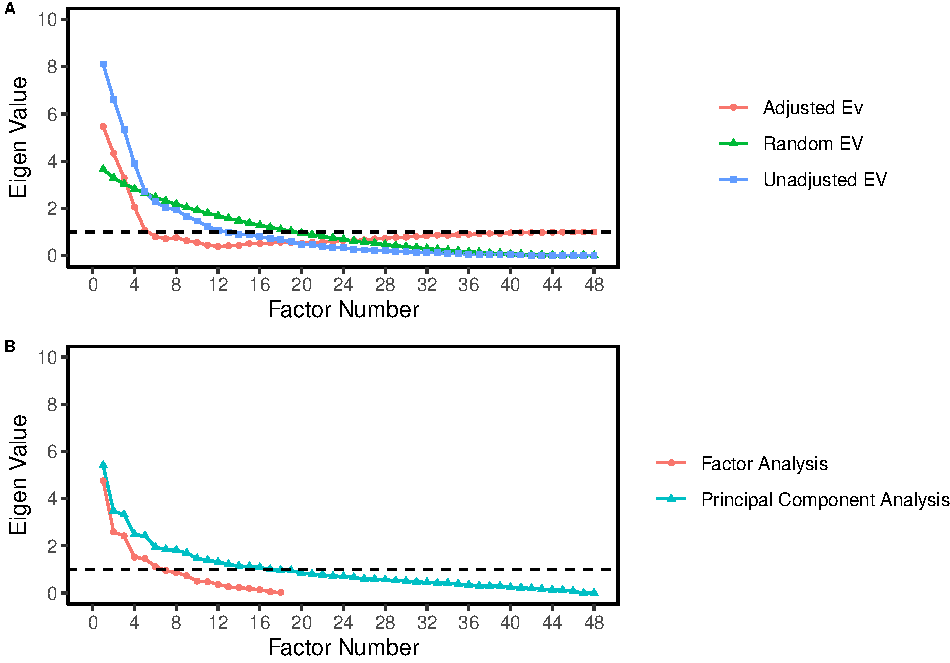
\includegraphics{manuscript_files/figure-latex/facIdFigAppB-1.pdf}
\caption{(\#fig:facIdFigAppB)Factor Identification (A) Parallel analysis
(B) Scree Plot {[}Unmerged response options{]}}
\end{figure}

\begin{center}
\begin{ThreePartTable}

\begin{TableNotes}[para]
\normalsize{\textit{Note.} Only loading higher than .30 is reported}
\end{TableNotes}

\begin{longtable}{llllllll}\noalign{\getlongtablewidth\global\LTcapwidth=\longtablewidth}
\caption{\label{tab:EFATableAppB}Factor loadings and communality of the retained items in five factor solution [Unmerged Responses]}\\
\toprule
item & \multicolumn{1}{c}{PA1} & \multicolumn{1}{c}{PA2} & \multicolumn{1}{c}{PA5} & \multicolumn{1}{c}{PA3} & \multicolumn{1}{c}{PA4} & \multicolumn{1}{c}{Communality} & \multicolumn{1}{c}{Uniqueness}\\
\midrule
\endfirsthead
\caption*{\normalfont{Table \ref{tab:EFATableAppB} continued}}\\
\toprule
item & \multicolumn{1}{c}{PA1} & \multicolumn{1}{c}{PA2} & \multicolumn{1}{c}{PA5} & \multicolumn{1}{c}{PA3} & \multicolumn{1}{c}{PA4} & \multicolumn{1}{c}{Communality} & \multicolumn{1}{c}{Uniqueness}\\
\midrule
\endhead
item19 & 0.99 &  &  &  &  & 1.007 & -0.007\\
item20 & 0.91 &  &  &  &  & 0.874 & 0.126\\
item18 & 0.82 &  &  &  &  & 0.711 & 0.289\\
item21 & 0.8 &  &  &  &  & 0.683 & 0.317\\
item4 & 0.47 &  &  &  &  & 0.25 & 0.75\\
item11 &  & 0.83 &  &  &  & 0.687 & 0.313\\
item10 &  & 0.81 &  &  &  & 0.67 & 0.33\\
item12 &  & 0.56 &  &  &  & 0.371 & 0.629\\
item8 &  & -0.44 &  &  &  & 0.206 & 0.794\\
item7 &  & 0.42 &  &  &  & 0.226 & 0.774\\
item9 &  & 0.33 &  &  &  & 0.115 & 0.885\\
item16 &  &  & 0.95 &  &  & 0.946 & 0.054\\
item17 &  &  & 0.74 &  &  & 0.595 & 0.405\\
item36 & 0.3 &  & 0.73 &  &  & 0.653 & 0.347\\
item3 &  &  &  & 0.85 &  & 0.746 & 0.254\\
item27 &  &  &  & 0.78 &  & 0.624 & 0.376\\
item40 &  &  &  & 0.71 &  & 0.512 & 0.488\\
item35 &  &  &  &  & 0.58 & 0.351 & 0.649\\
item48 &  &  &  &  & 0.57 & 0.354 & 0.646\\
item33 &  &  &  &  & 0.55 & 0.32 & 0.68\\
item47 &  &  &  &  & 0.52 & 0.294 & 0.706\\
item44 &  &  &  &  & 0.45 & 0.216 & 0.784\\
item31 &  &  &  &  & 0.41 & 0.206 & 0.794\\
item38 &  &  &  &  & 0.33 & 0.129 & 0.871\\
\% of Variance & 0.15 & 0.09 & 0.09 & 0.08 & 0.08 &  & \\
\bottomrule
\addlinespace
\insertTableNotes
\end{longtable}

\end{ThreePartTable}
\end{center}

\begin{center}
\begin{ThreePartTable}

\begin{TableNotes}[para]
\normalsize{\textit{Note.} Only loading higher than .30 is reported}
\end{TableNotes}

\begin{longtable}{lllllllll}\noalign{\getlongtablewidth\global\LTcapwidth=\longtablewidth}
\caption{\label{tab:EFAsix}Factor loadings and communality of the retained items in six factor solution [Unmerged Responses]}\\
\toprule
item & \multicolumn{1}{c}{PA1} & \multicolumn{1}{c}{PA2} & \multicolumn{1}{c}{PA3} & \multicolumn{1}{c}{PA4} & \multicolumn{1}{c}{PA6} & \multicolumn{1}{c}{PA5} & \multicolumn{1}{c}{Communality} & \multicolumn{1}{c}{Uniqueness}\\
\midrule
\endfirsthead
\caption*{\normalfont{Table \ref{tab:EFAsix} continued}}\\
\toprule
item & \multicolumn{1}{c}{PA1} & \multicolumn{1}{c}{PA2} & \multicolumn{1}{c}{PA3} & \multicolumn{1}{c}{PA4} & \multicolumn{1}{c}{PA6} & \multicolumn{1}{c}{PA5} & \multicolumn{1}{c}{Communality} & \multicolumn{1}{c}{Uniqueness}\\
\midrule
\endhead
item19 & 0.98 &  &  &  &  &  & 0.995 & 0.005\\
item20 & 0.92 &  &  &  &  &  & 0.904 & 0.096\\
item21 & 0.79 &  &  &  &  &  & 0.666 & 0.334\\
item4 & 0.49 &  &  &  &  &  & 0.296 & 0.704\\
item43 & 0.32 &  &  &  &  & 0.31 & 0.282 & 0.718\\
item10 &  & 0.81 &  &  &  &  & 0.67 & 0.33\\
item11 &  & 0.81 &  &  &  &  & 0.668 & 0.332\\
item12 &  & 0.58 &  &  &  &  & 0.408 & 0.592\\
item8 &  & -0.45 &  &  &  &  & 0.218 & 0.782\\
item7 &  & 0.42 &  &  &  &  & 0.229 & 0.771\\
item9 &  & 0.33 &  &  &  &  & 0.115 & 0.885\\
item3 &  &  & 0.85 &  &  &  & 0.731 & 0.269\\
item27 &  &  & 0.77 &  &  &  & 0.606 & 0.394\\
item40 &  &  & 0.72 &  &  &  & 0.533 & 0.467\\
item35 &  &  &  & 0.64 &  &  & 0.426 & 0.574\\
item33 &  &  &  & 0.62 &  &  & 0.413 & 0.587\\
item48 &  &  &  & 0.52 &  &  & 0.305 & 0.695\\
item47 &  &  &  & 0.48 &  &  & 0.259 & 0.741\\
item31 &  &  &  & 0.39 &  &  & 0.206 & 0.794\\
item38 &  &  &  & 0.32 &  &  & 0.18 & 0.82\\
item17 &  &  &  &  & 0.85 &  & 0.786 & 0.214\\
item16 &  &  &  &  & 0.78 &  & 0.681 & 0.319\\
item13 &  &  &  &  &  & 0.57 & 0.336 & 0.664\\
item14 &  &  &  &  &  & 0.5 & 0.356 & 0.644\\
item15 &  &  &  &  &  & 0.48 & 0.277 & 0.723\\
item42 &  &  &  &  &  & 0.37 & 0.168 & 0.832\\
item26 &  &  &  &  &  &  & 0.064 & 0.936\\
\% of Variance & 0.11 & 0.08 & 0.07 & 0.06 & 0.06 & 0.05 &  & \\
\bottomrule
\addlinespace
\insertTableNotes
\end{longtable}

\end{ThreePartTable}
\end{center}

\hypertarget{items-retained-in-the-five-factor-solution-unmerged-responses}{%
\section{Items Retained in the Five Factor Solution {[}Unmerged
Responses{]}}\label{items-retained-in-the-five-factor-solution-unmerged-responses}}

\begin{longtable}[]{@{}
  >{\raggedright\arraybackslash}p{(\columnwidth - 0\tabcolsep) * \real{1.00}}@{}}
\toprule
\begin{minipage}[b]{\linewidth}\raggedright
\textbf{Five Factor Solution {[}Unmerged Responses{]} (24 Items)}
\end{minipage} \\
\midrule
\endhead
\textbf{F1} \\
I use light therapy applying a blue light box. \\
I use light therapy applying a light visor. \\
I use light therapy applying a white light box. \\
I use light therapy applying another form of light device. \\
I use an alarm with a dawn simulation light. \\
\textbf{F2} \\
I spend more than 3 hours per day (in total) outside. \\
I spend between 1 and 3 hours per day (in total) outside. \\
I spend as much time outside as possible. \\
I spend 30 minutes or less per day (in total) outside. \\
I go for a walk or exercise outside within 2 hours after waking up. \\
I spend between 30 minutes and 1 hour per day (in total) outside. \\
\textbf{F3} \\
I look at my mobile phone screen immediately after waking up. \\
I use my mobile phone within 1 hour before attempting to fall asleep. \\
I check my phone when I wake up at night. \\
\textbf{F4} \\
I use a blue-filter app on my computer screen within 1 hour before
attempting to fall asleep. \\
I seek out knowledge on how to improve my light exposure. \\
I dim my computer screen within 1 hour before attempting to fall
asleep. \\
I discuss the effects of light on my body with other people. \\
I modify my light environment to match my current needs. \\
I dim my room light within 1 hour before attempting to fall asleep. \\
I use as little light as possible when I get up during the night. \\
\textbf{F5} \\
I wear blue-filtering, orange-tinted, and/or red-tinted glasses indoors
during the day. \\
I wear blue-filtering, orange-tinted, and/or red-tinted glasses outdoors
during the day. \\
I wear blue-filtering, orange-tinted, and/or red-tinted glasses within 1
hour before attempting to fall asleep. \\
\bottomrule
\end{longtable}
\end{appendix}
